%%%%%%%%%%%%%%%%%%%%%%%%%% ch2-StochasticProcess
\begin{frame}[shrink]
\frametitle{ch2.信号检测与估计理论的基础知识}
\framesubtitle{随机过程}
\tableofcontents[hideallsubsections]
\end{frame}

\section{随机过程的定义}

\begin{frame}{随机过程引例(1)}
\begin{example}
	考察$[0,t_0]$时间内某网站收到的访问次数$X(t_0)$, $X(t_0)$则是一个随机变量。
	\begin{itemize}
		\item 如果要长时间内该网站的访问次数,则需要让$t$变化起来,即$t$趋于无穷大,则$X(t)$是一簇随机变量.
		\item 此时$X(t)$是与时间有关系的随机变量, 称$\{X(t),t\in[0,\infty]\}$是随机过程。
	\end{itemize}	
\end{example}
\end{frame}

\begin{frame}{随机过程引例(2)}
\begin{example}
	具有随机初位相的简谐波
	\[X(t)=A\cos(\omega t+\Phi)\]
	其中$A,\omega$为常数,$\Phi$服从$[0,2\pi]$上的均匀分布。
	\begin{itemize}
		\item 由于初位相的随机性,在某时刻$t=t_0,X(t)$是一个随机变量.
		\item 若要观察任一时刻$t$的波形,则需要用一簇随机变量$X(t)$描述. 
		\item 称$\{X(t),t\in[0,\infty]\}$是随机过程。
	\end{itemize}	
\end{example}
\end{frame}

\begin{frame}{随机过程引例(3)}
\begin{columns}
	\column{0.6\textwidth}
	\begin{example}
		每次热噪声电压测量结果:固定$t$时刻电压,对应一个随机变量$v(t)$; \\
		无限个$t$,则无限个电压---时间的函数族构成一随机过程。
	\end{example}
	\column{0.4\textwidth}
	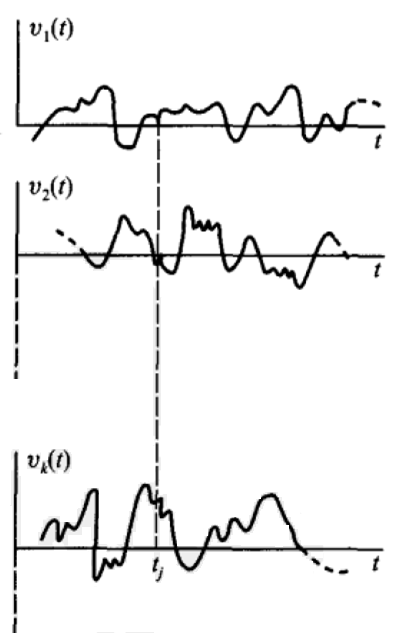
\includegraphics[scale=0.3]{vt}
\end{columns}
\end{frame}

\begin{frame}{随机过程引例(4)}
\begin{example}
	生物群体的增长问题.以$X_t$表示在时刻$t$某种生物群体的个数,则对每一个固定的$t,X_t$是一个随机变量。 
	\begin{itemize}
		\item 如果从$t=0$开始,每隔24小时对群体的个数观察一次,则对每一个$t$,$X_t$是一簇随机变量。记为$X_n,n=0,1,\dots$
		\item 若要观察任一时刻$t$的波形,则需要用一族随机变量$X(t)$描述. 
		\item 称$\{X_t,t=0,1,2,\dots\}$是随机过程。
	\end{itemize}	
\end{example}
\end{frame}

\begin{frame}{随机过程引例特点}
\begin{block}{以上例子的共同特点---随机现象在时间上的延展$\implies$\textbf{随机过程$\{X(t,\xi),t\in T,\xi\in \Omega\}$}}
	\begin{itemize}
		\item 给定一个$t$,就有\textbf{一个随机变量$X(t)$}与之对应。
		\item 概率论主要是以\textbf{一个或有限个随机变量}为研究对象的.
		\item 随机过程是概率论的``动力学''部分,研究对象为随时间演变的随机现象,通常会有\textbf{无穷多个随机变量}。
	\end{itemize}
\end{block}
\begin{columns}
	\column{0.4\textwidth}
	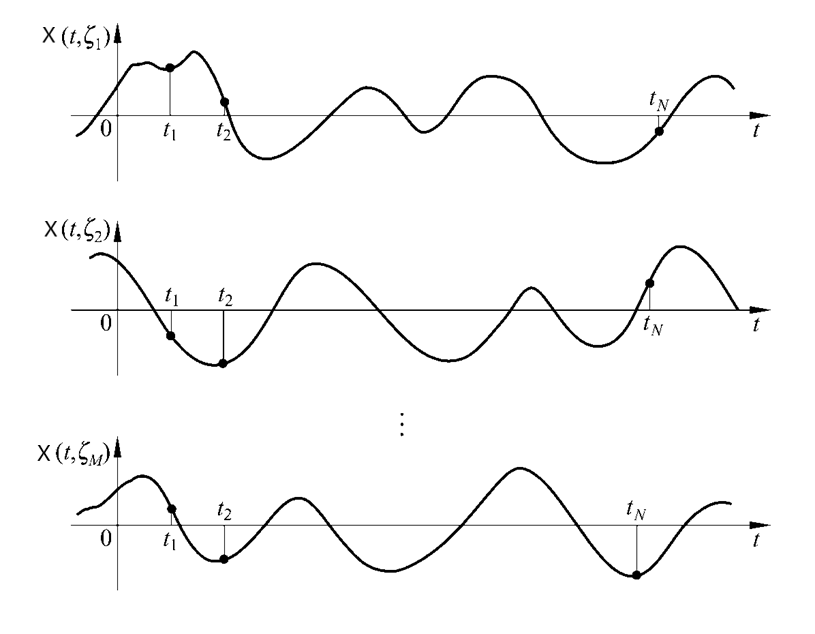
\includegraphics[scale=0.2]{sampleFun}
	\column{0.6\textwidth}
	\small
	$X(t_1)=\{X(t_1,\xi_1), X(t_1,\xi_2),\cdots, X(t_1,\xi_M)\}$	\\
	$X(t_2)=\{X(t_2,\xi_1), X(t_2,\xi_2),\cdots, X(t_2,\xi_M)\}$	\\
	$\qquad\qquad\vdots\qquad\qquad\qquad\vdots$\\
	$X(t_N)=\{X(t_N,\xi_1), X(t_N,\xi_2),\cdots, X(t_N,\xi_M)\}$\\
	\textcolor{blue}{$M$次试验, 每次进行$N$次采样, $N$个随机变量$X_{t}$。}
\end{columns}	
\end{frame}

\begin{frame}%{随机过程的定义}
\begin{definition}[随机过程]
	设$(\Omega,\mathcal{F},P)$是一概率空间, $T$是一实参数集,定义在$\Omega$和$T$上的二元函数$X(t,\xi)$
	\begin{enumerate}
		\item 固定$t_k\in T,X(t_k,\xi)$是概率空间上的\textbf{随机变量};
		\item 固定$\xi_i\in\Omega,X(t,\xi_i)$是概率空间上的\textbf{随机函数}(或称$X(t,\xi_i)$是对应于$\xi_i$的\textbf{样本函数})
	\end{enumerate}
    则称$\{X(t,\xi),t\in T,\xi\in \Omega \}$为一\textbf{随机过程},简记为$X(t)$,其中$t$和$\xi$均是变量。\\
	随机过程的定义域是实参数集$T$和样本空间$\Omega$。值域是实数集$\mathbb{R}$.
	\begin{itemize}
		\item \textbf{样本空间$\Omega$}:一个随机试验所有可能出现的结果的全体,称为随机事件的样本空间。\\
		\item 事件域$\mathcal{F}$: 样本空间中的某些子集。
		\item
		\textbf{参数集$T$}: 表示时间或空间,通常的形式: $T=\{0,1,2,\dots \}$或$T=[a,b],T=(-\infty,\infty)$
	\end{itemize}
	\end{definition}
\end{frame}

\begin{frame}{用映射表示随机过程} 
\begin{columns}
	\column{0.2\textwidth}
	\small
	\[X(t,\xi): T\times\Omega\to\mathbb{R} \]
	\column{0.25\textwidth}
	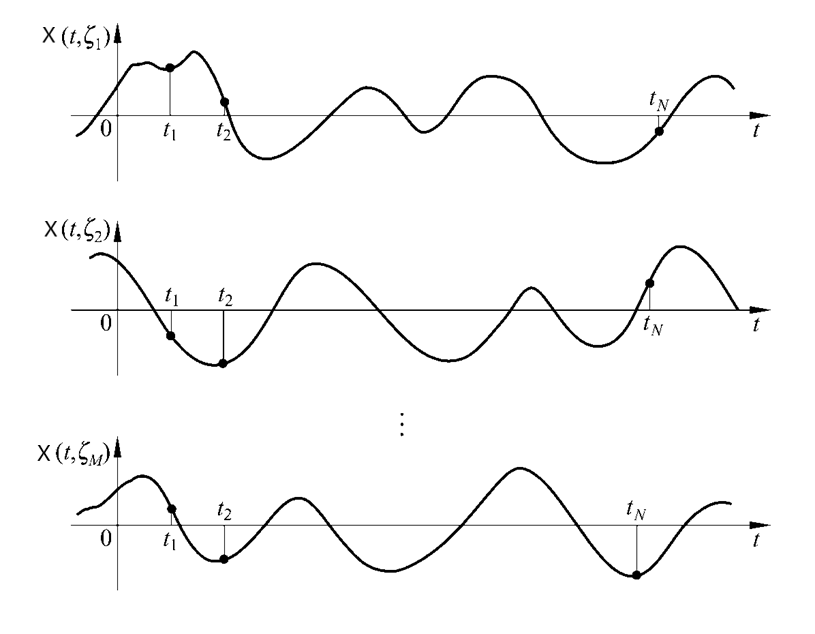
\includegraphics[scale=0.15]{sampleFun}
	\column{0.55\textwidth}
	\small
	$X(t_1,\bullet)=\{X(t_1,\xi_1), X(t_1,\xi_2),\cdots, X(t_1,\xi_M)\}$	\\
	$X(t_2,\bullet)=\{X(t_2,\xi_1), X(t_2,\xi_2),\cdots, X(t_2,\xi_M)\}$	\\
	$\qquad\qquad\vdots\qquad\qquad\qquad\vdots$\\
	$X(t_N,\bullet)=\{X(t_N,\xi_1), X(t_N,\xi_2),\cdots, X(t_N,\xi_M)\}$
\end{columns}
\begin{enumerate}
	\item $X(\bullet,\bullet)$实质是定义在$T\times\Omega$上的二元单值函数;
	\item 固定$t\in T,X(t,\bullet)$是样本空间$\Omega$上的函数,即$X(t,\bullet)$为一\textbf{随机变量};
	\item 固定$\xi\in\Omega,X(\bullet,\xi)$是一个关于$t\in T$的函数,通常称为\textbf{样本函数},或称随机过程的\textbf{一次实现},所有样本函数的集合确定一随机过程。
	\item 随机过程$\{X(t,\xi)\}$可能取值的全体所构成的集合称为此随机过程的\textbf{状态空间},记作$S$。$S$中的元素称为\textbf{状态}。状态空间可以由复数、实数或更一般的抽象空间构成。
\end{enumerate}
\textcolor{blue}{记号$X(t,\xi)$有时记为$X_t(\xi)$或简记为$X(t)$。}
\end{frame}

\begin{frame}
\begin{example}[随机过程示例]
	抛掷硬币的试验,样本空间$\Omega=\{H,T\}$, 定义
	\[X(t)=\begin{cases}
	\cos\pi t, &\text{当出现$H$}\\
	t, &\text{当出现$T$}\\ 
	\end{cases}, t\in(-\infty,\infty)\]
	其中$P(H)=P(T)=1/2$, 则$\{X(t), t\in (-\infty, +\infty)\}$是一随机过程。试考察其样本函数和状态空间。
\end{example}

\medskip
\begin{columns}
	\column{0.4\textwidth}
	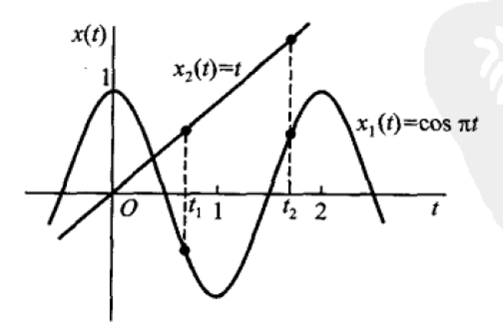
\includegraphics[scale=0.32]{sin_t}
	\column{0.6\textwidth}
	样本函数: $X(\bullet,\xi)=\{\cos\pi t, t\}, \xi\in \Omega$\\
	状态空间: $S=\{\cos\pi t_0, t_0\}, \forall t_0\in (-\infty, +\infty)$\\
	每次试验的结果是下列事件集合之一:
	\[ \{(H,T),(T,H),(H,H),(T,T)\} \]
\end{columns}
\end{frame}

\begin{frame}
\begin{example}
	考察$[0,t_0]$时间内某网站收到的访问次数$X(t_0)$, $X(t_0)$则是一个随机变量。
	\begin{itemize}
		\item 如果要长时间内该网站的访问次数,则需要让$t$变化起来,即$t$趋于无穷大,则$X(t)$是一簇随机变量.
		\item 此时$X(t)$是与时间有关系的随机变量, 称$\{X(t),t\in[0,\infty)\}$是随机过程。
	\end{itemize}
\end{example}
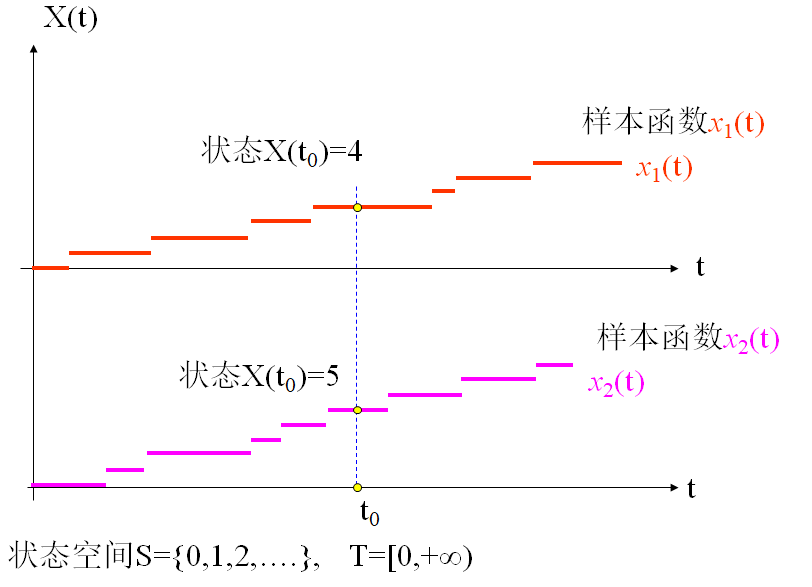
\includegraphics[scale=0.2]{sampleFun1}	
\end{frame}

\begin{frame}
\begin{example}
具有随机初位相的简谐波
\[X(t)=A\cos(\omega t+\Phi)\]
其中$A,\omega$为常数,$\Phi$服从$[0,2\pi]$上的均匀分布。
\begin{itemize}
	\item 由于初位相的随机性,在某时刻$t=t_0,X(t)$是一个随机变量.
	\item 若要观察任一时刻$t$的波形,则需要用一簇随机变量$X(t)$描述. 
	\item 称$\{X(t),t\in[0,\infty)\}$是随机过程。
\end{itemize}	
\end{example}
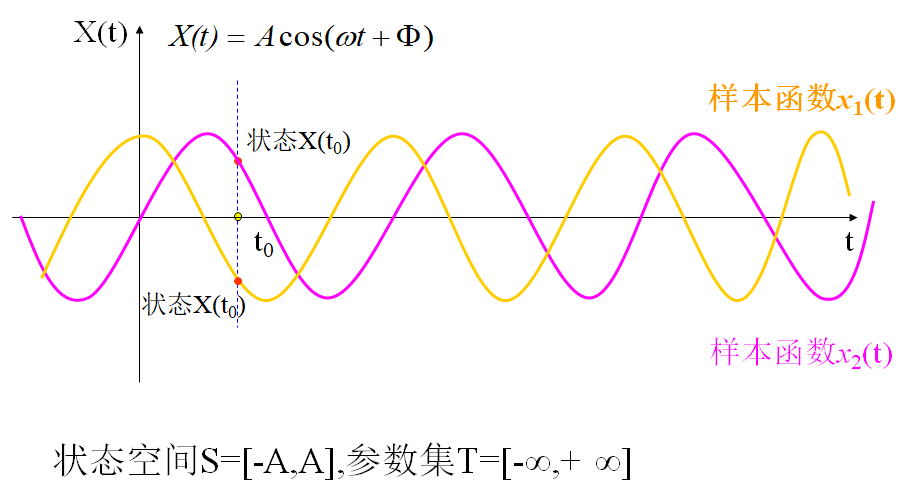
\includegraphics[scale=0.2]{sampleFun2}	
\end{frame}

\begin{frame}
\begin{columns}
\column{0.7\textwidth}
\begin{example}
每次热噪声电压测量结果:固定$t$时刻电压,对应一个随机变量$v(t)$; \\
无限个$t$,则无限个电压---时间的函数族$\{v(t),t\in[0,\infty)\}$构成一随机过程。\\
\end{example}
对某种装置做一次试验,便得到一个电压---时间函数$v_1(t)$。这个电压---时间函数是不可能预先确知的,只有通过测量才能得到,如果在相同的条件下独立地再进行一次测量,则得到的记录是不同的。\\

\medskip
样本函数: $X(\bullet,\xi)=\{v_k(t)\}, k=1,2,\dots, \xi\in \Omega$\\
状态空间: $S=\{v_k(t_0)\}, k=1,2,\dots, \forall t_0\in (-\infty, +\infty)$
\column{0.3\textwidth}
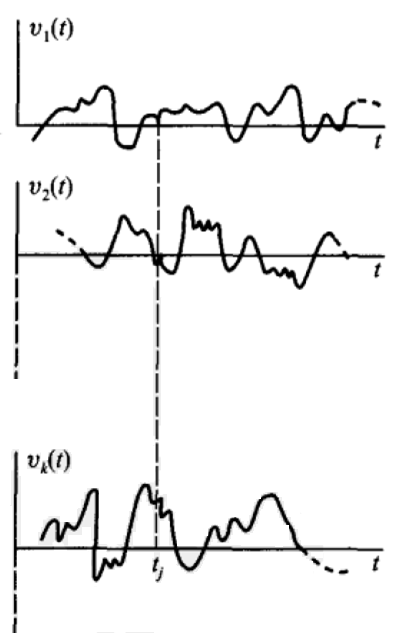
\includegraphics[scale=0.3]{vt}
\end{columns}
\end{frame}

\begin{frame}
\begin{example}
生物群体的增长问题.以$X_t$表示在时刻$t$某种生物群体的个数,则对每一个固定的$t,X_t$是一个随机变量。 
\begin{itemize}
\item 如果从$t=0$开始,每隔24小时对群体的个数观察一次,则对每一个$t$,$X_t$是一簇随机变量。记为$X_n,n=0,1,\dots$
\item 若要观察任一时刻$t$的波形,则需要用一族随机变量$X(t)$描述. 
\item 称$\{X_t,t=0,1,2,\dots\}$是随机过程。
\end{itemize}	
\end{example}
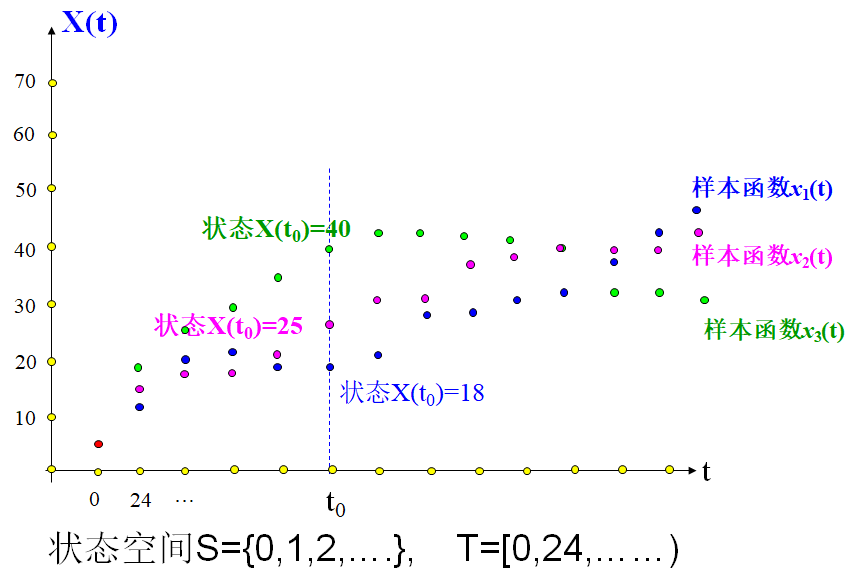
\includegraphics[scale=0.15]{sampleFun3}	
\end{frame}

\begin{frame}
\begin{example}
	设随机相位正弦信号$s(t; \theta)=a\cos(\omega_0 t+\theta)$, 其中振幅$a$和$\omega_0$为常数, 相位$\theta$是一随机变量,它服从$[-\pi,\pi]$上的均匀分布。写出$s(t;\theta)$的样本函数。
\end{example}
解: \\
当$\theta$在$[-\pi,\pi]$内任取定值时,如\\
当$\theta=0$, 则样本函数为
$$s_1(t; \theta=0)=a\cos\omega_0t$$
当$\theta=\frac{\pi}{2}$, 则样本函数为
$$s_2(t; \theta=\frac{\pi}{2})=a\cos(\omega_0t+\frac{\pi}{2})=-a\sin\omega_0t$$
\end{frame}

\section{随机过程的统计描述}

\begin{frame}{一维概率密度函数}
连续随机过程$\{X(t,\xi),t\in T,\xi\in\Omega \}$的$M$个样本函数如图。通常用\textbf{有限维概率密度函数}来描述随机过程。

\medskip
\begin{columns}
	\column{0.6\textwidth}
	\begin{block}{}
		%\small
		设$\{X(t,\xi),t\in T,\xi\in\Omega \}$是一随机过程,对于任意固定的时刻$t,X(t,\xi)$是一随机变量,称
		\[F(x;t)=P\{X(t,\xi)\le x\},x\in\mathbb{R},t\in T \]
		为该随机过程的\textbf{一维累积分布函数}。\\
		如果$F(x;t)$对$x$的一阶导数存在,则有
		\[p(x;t)=\frac{dF(x;t)}{dx}\]
		$p(x;t)$为随机过程$X(t,\xi)$的\textbf{一维概率密度函数}。
	\end{block}
	\column{0.4\textwidth}
	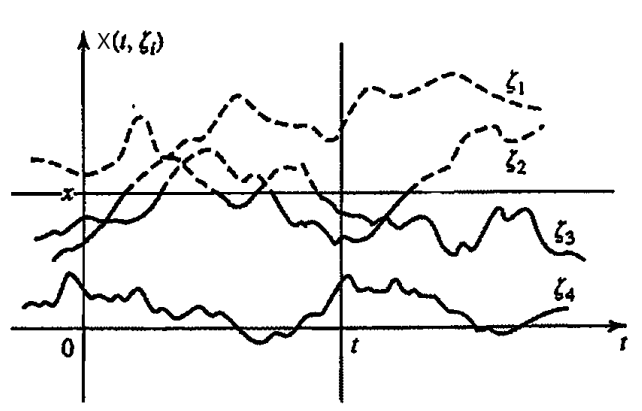
\includegraphics[scale=0.3]{sampleFun4}
\end{columns}
\end{frame}

\begin{frame}{二维联合概率密度函数}
对于任意固定的时刻$t_1,t_2\in T$, 随机变量$X(t_1,\xi),X(t_2,\xi)$构成二维矢量$[X(t_1,\xi),X(t_2,\xi)]^T$,称
\[F(x_1,x_2;t_1,t_2)=P\{X(t_1,\xi)\le x_1,X(t_2,\xi)\le x_2\},x_1,x_2\in\mathbb{R},t_1,t_2\in T \]
为该随机过程的\textbf{二维累积分布函数}。\\
如果$F(x_1,x_2;t_1,t_2)\in T$对$x_1,x_2$的二阶混合偏导数存在,则有
\[p(x_1,x_2;t_1,t_2)=\frac{\partial^2 F(x_1,x_2;t_1,t_2)}{\partial x_1\partial x_2}\]
$p(x;t)$称为随机过程$X(t,\xi)$的\textbf{二维联合概率密度函数}。
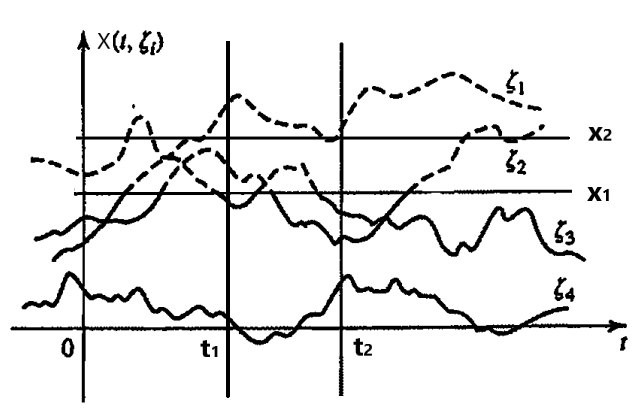
\includegraphics[scale=0.23]{sampleFun4-2}
\end{frame}

\begin{frame}{N维联合概率密度函数}
推广至N维随机矢量的情况\\
随机过程的\textbf{N维累积分布函数}
\begin{align*}
F(x_1,x_2,\cdots,x_N;t_1,t_2,\cdots,t_N)&=\\
&P\{X(t_1,\xi)\le x_1,X(t_2,\xi)\le x_2,\cdots,X(t_N,\xi)\le x_N\},&\\
&x_1,x_2,\cdots,x_N\in\mathbb{R},t_1,t_2,\cdots,t_N\in T
\end{align*}
随机过程的\textbf{N维联合概率密度函数}
\begin{align*}
p(x_1,x_2,\cdots,x_N;t_1,t_2,\cdots,t_N)&=\\
&\frac{\partial^N F(x_1,x_2,\cdots,x_N;t_1,t_2,\cdots,t_N)}{\partial x_1\partial x_2\cdots\partial x_N}
\end{align*}
\end{frame}

\begin{frame}{一维雅可比变换法}
设一维随机变量为$X(\xi)$,它的概率密度函数为$p_x(x)$已知,若$X(\xi)$的一个函数为
\[Y(\xi)=g(X(\xi)) \]
该函数也是一维随机变量。若它的反函数存在,即有
\[X(\xi)=h(Y(\xi)) \]
且连续可导,则$Y(\xi)$的概率密度函数为
\[p_y(y)=p_x[x=h(y)]|J| \]
这种变换称为\textbf{一维雅可比变换},其中\textbf{雅可比}$J=\frac{dh(Y)}{dY}$, $|\bullet|$是绝对值符号。
\begin{block}{Notes}
	$Y(\xi)$的概率密度函数$p_y(y)$可以通过它的反函数$X(\xi)$的概率密度函数$p_x(x)$与雅可比的乘积得到。
\end{block}
\end{frame}

\begin{frame}
\begin{example}
	设随机过程$X(t)=V\cos\omega t,t\in(-\infty,+\infty)$, 其中$\omega$为常数, $V$服从$[0,1]$上的均匀分布。
	\begin{enumerate}
		\item 确定$\{X(t),t\in(-\infty,+\infty)\}$的两个样本函数。
		\item 求$t=0,t=3\pi/4\omega$时,随机变量$X(t)$的概率密度函数。
		\item 求$t=\pi/2\omega$时, $X(t)$的分布函数。
	\end{enumerate}
\end{example}
\end{frame}

\begin{frame}
设随机过程$X(t)=V\cos\omega t,t\in(-\infty,+\infty)$, 其中$\omega$为常数, $V$服从$[0,1]$上的均匀分布。\\
解: 
\begin{enumerate}
	\item $V\sim U(0,1)$, 取$V=1/2,1/3$分别得到两个样本函数
	\[X_1(t)=\frac{1}{2}\cos\omega t,\qquad X_2(t)=\frac{1}{3}\cos\omega t\]
	\item $t=0$时, $X(t)=V\cos\omega 0=V$,而$V$为$[0,1]$上的均匀分布,则
	$$
	p(x;t=0)=\begin{cases}
	1 & 0\le x\le 1\\
	0 &\text{其它}	
    \end{cases}
    $$
\end{enumerate}
\end{frame}

\begin{frame}
解(续):
\begin{enumerate}
	\setcounter{enumi}{1} %设定起始编号 
	\item (续) 当$t=\frac{3\pi}{4\omega}$时,$X(t)=V\cos\omega\frac{3\pi}{4\omega}=-\frac{\sqrt{2}}{2}V$\\
	由于函数$x=-\frac{\sqrt{2}}{2}V$的反函数为$V=h(x)=-\sqrt{2}x$,其导数为$h^\prime(x)=-\sqrt{2}$,则利用一维雅可比变换公式,求得
	\begin{align*}
		p(x,t=\frac{3\pi}{4\omega}) &=\begin{cases}
		p_V(h(x))|h^\prime(x)| &0\le h(x)\le 1\\
		0 &\text{其它}
		\end{cases}\\
		&=\begin{cases}
		\sqrt{2} &0\le -\sqrt{2}x\le 1\\
		0 &\text{其它}
		\end{cases}\\
		&=\begin{cases}
		\sqrt{2} &\frac{-\sqrt{2}}{2}\le x\le 0\\
		0 &\text{其它}
		\end{cases}
	\end{align*}
\end{enumerate}
\end{frame}

\begin{frame}
解(续):
\begin{enumerate}
	\setcounter{enumi}{2} %设定起始编号 
	\item $t=\frac{\pi}{2\omega}$时,$X(t)=V\cos\omega\frac{\pi}{2\omega}=0$, 此时$X(t=\frac{\pi}{2\omega})$是单点分布,则
	\begin{align*}
	F(x,t=\frac{\pi}{2\omega}) &=P\{X(t)\le x \}\\
	&=\begin{cases}
	1 &x\ge 0\\
	0 &x<0
	\end{cases}
	\end{align*}
\end{enumerate}
\end{frame}

\begin{frame}
\begin{example}
设有一采用脉宽调制以传输信息的通信系统。脉冲的重复周期为$T$,每个周期传输一个值, 脉冲宽度收到随机信息的调制,使每个脉冲的宽度$\tau$服从$(0,T)$上的均匀分布,而且不同周期的脉宽是相互统计独立的随机变量。脉冲的幅度为常数$A$。 也就是说,这个通信系统传送的信号是随机脉宽等幅度的周期信号,它是一个随机过程。下图画出了它的一个样本函数。试求该随机过程$X(t)$的一维概率密度函数。
\end{example}
\begin{figure}
	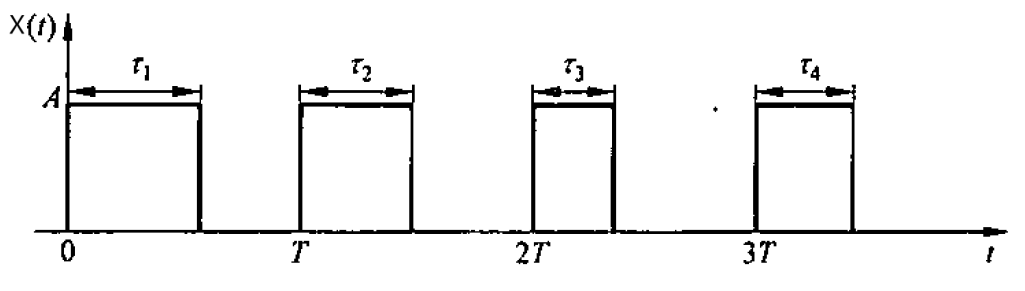
\includegraphics[scale=0.3]{2_10SampleFun}
	\caption {脉宽调制信号的一个样本函数}
\end{figure}
\end{frame}

\begin{frame}[shrink]
\begin{example}[解]
	因为脉冲的重复周期为$T$,所以只需求出一个周期的概率密度函数。\\
	在一个周期内,随机信号为
	\[
	X(t)=\begin{cases}
	A,&0\le t\le\tau\\
	0,&\tau<t\le T
	\end{cases} 
	\]
	$X(t)$的分布函数为
	\[
	F(x;t)=P\{X(t)\le x \}=\begin{cases}
	0,&x<0\\
	\frac{t}{T},&0\le x<A\\
	1,&x\ge A
	\end{cases} 
	\]
	所以,它的一维概率密度函数为:
	\[p(x;t)=\frac{t}{T}\delta(x)+(1-\frac{t}{T})\delta(x-A) \]
\end{example}
\small
由$\delta$函数性质, 当$x=0$时, $\delta(x)=\infty$; 其它, $\delta(x)=0$. 并且$\int_{-\infty}^{\infty}\delta(x)dx=1$\\
可以验证以上分布函数的正确性.  $F(x; t)=P\{X(t)\le x\}=\int_{-\infty}^{x}p(u)du$
\end{frame}

%\section{随机过程的统计平均量}

\begin{frame}
连续函数$f(x)$在区间$[a,b]$的均值:
\[\bar{y}=\frac{1}{b-a}\lim\limits_{\Delta x\to 0}\sum\limits_{i=1}^{n}f(x_{i-1})\Delta x=\frac{1}{b-a}\int_{a}^{b}f(x)dx \]
交流电$I(t)=I_m\sin\omega t$, 其平均值表示它的直流分量: $\overline{I}=\frac{1}{T}\int_{0}^{T}I(t)dt$\\
电压$U(t)=iR=I_mR\sin\omega t$, , 其平均值表示它的直流分量: $\overline{U}=\frac{1}{T}\int_{0}^{T}U(t)dt$\\
功率$p=U(t)I(t)=I_m^2R\sin^2\omega t$\\
此功率在长度为一个周期的区间$[0,\frac{2\pi}{\omega}]$上的平均值:
\[\bar{p}=\frac{1}{\frac{2\pi}{\omega}}\int_{0}^{\frac{2\pi}{\omega}}I_m^2R\sin^2\omega tdt=\frac{I_m^2R}{2}=\frac{I_mU_m}{2},(U_m=I_mR) \]
$I_m,U_m$为交流电电流、电压的最大值,$\omega$为交流电的角频率。
\end{frame}

\begin{frame}
以下用记号$\{x(t),t\in T\}$表示随机过程, 固定$t\in T, x(t)$是一随机变量。
\begin{block}{随机过程的均值$\mu_x(t)$: 表示随机过程在$t$时刻状态取值的\textbf{理论平均值}}
	\[\mu_x(t)\mathop{=}^{def}E[x(t)]=\int_{-\infty}^{\infty}xp(x;t)dx \]
	如果$x(t)$是电压或电流,则$\mu_x(t)$可以理解为在$t$时刻的``直流分量''。\\
	随机过程$x(t)$的均值又称作数学期望(Expectation)。$\mu_x(t)$是随机过程的\textbf{所有样本函数}在时刻$t$的函数值的统计平均值。$\mu_x(t)$表示了随机过程$x(t)$在各个时刻的摆动中心。
\end{block}

\begin{block}{Notes}
	\begin{itemize}
		\item 如果$y(t)=g(x(t))$, 则$\mu_y(t)=E[g(x(t))]=\int_{-\infty}^{\infty}g(x)p_x(x)dx$
		\item 均值的线性特性: $y(t)=ax(t)+b$, \quad $a,b$为常数, 则$\mu_y(t)=E[y(t)]=E[ax(t)+b]=aE[x(t)]+b=a\mu_x(t)+b$
	\end{itemize}
\end{block}
\end{frame}

\begin{frame}
\begin{block}{随机过程的均方值$\varphi_x^2(t)$}
	\[\varphi_x^2(t)\mathop{=}^{def}E[x^2(t)]=\int_{-\infty}^{\infty}x^2p(x;t)dx \]
	如果$x(t)$是电压或电流,则$\varphi_x^2(t)$可以理解在$t$时刻它在$1\Omega$电阻上消耗的``平均功率''。
\end{block}
\begin{block}{随机过程的方差/标准偏差$\delta_x^2(t)$}
\[\sigma_x^2(t)\mathop{=}^{def}E[(x(t)-\mu_x(t))^2]=\int_{-\infty}^{\infty}(x-\mu_x(t))^2p(x;t)dx \]
方差$\sigma_x^2(t)$表示随机过程在$t$时刻取其值\textbf{偏离其均值}$\mu_x(t)$的离散程度。\\
如果$x(t)$是电压或电流,$\delta_x^2(t)$表示在$t$时刻它在$1\Omega$电阻上消耗的``交流功率''。\\
随机过程$x(t)$的方差(Variance)有时用$Var[x(t)]$表示。
\end{block}
\end{frame}

\begin{frame}{均匀分布随机变量$x$的均值$\mu_x$和方差$\sigma_x^2$}
\begin{example}
	求如图均匀分布随机变量$x$的均值$\mu_x$和方差$\sigma_x^2$。
\end{example}
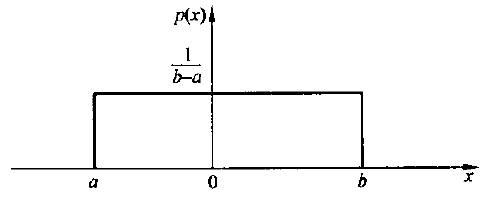
\includegraphics[scale=0.3]{ex2-1}
\end{frame}

\begin{frame}{均匀分布随机变量$x$的均值$\mu_x$和方差$\sigma_x^2$}
解: 随机变量$x$的概率密度函数$p(x)$为
\[p(x)=\begin{cases}
\frac{1}{b-a}, &a\le x\le b\\
0, &\text{其他}
\end{cases} \]

根据随机变量均值的定义,有
\begin{align*}
\mu_x=E(x)&=\int_{-\infty}^{\infty}xp(x)dx=\int_{a}^{b}\frac{1}{b-a}xdx =\frac{a+b}{2}
\end{align*}
根据随机变量方差的定义,有
\begin{align*}
\sigma_x^2=E[(x-\mu_x)^2]&=\int_{-\infty}^{\infty}(x-\mu_x)^2p(x)dx=\int_{a}^{b}\left(x-\frac{a+b}{2}\right)^2\frac{1}{b-a}dx \\
&=\frac{(b-a)^2}{12}
\end{align*}	
\end{frame}

\begin{frame}
\begin{block}{随机过程的自相关函数$r_x(t_j,t_k)$}
\begin{align*}
r_x(t_j,t_k)&\mathop{=}^{def}E[x(t_j)x(t_k)]\\
&=\int_{-\infty}^{\infty}	\int_{-\infty}^{\infty}x_jx_kp(x_j,x_k;t_j,t_k)dx_jdx_k
\end{align*}
\end{block}
随机过程的自相关函数$r_x(t_j,t_k)$可以理解为它的两个随机变量$x(t_j)$与$x(t_k)$之间\textbf{含有均值}时的相关程度的度量。显然
\[r_x(t,t)=\varphi_x^2(t)\]
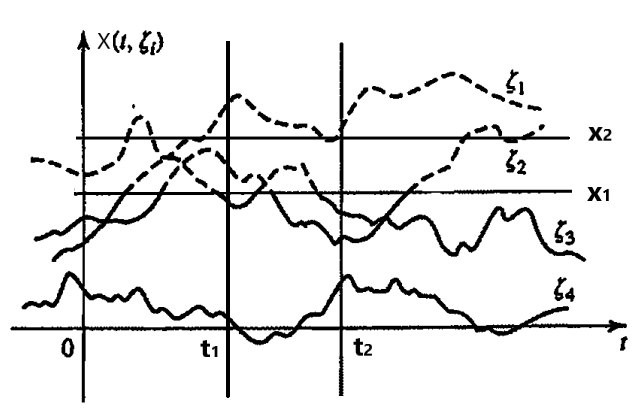
\includegraphics[scale=0.23]{sampleFun4-2}
\end{frame}

\begin{frame}
\begin{example}
	设随机过程$x(t)$的均值为$\mu_x(t)$,自相关函数为$r_x(t_j,t_k)$。若有随机过程$y(t)=a(t)x(t)+b(t)$, 其中$a(t),b(t)$是确知函数。求随机过程$y(t)$的均值和自相关函数。
\end{example}
\end{frame}

\begin{frame}
解:\\
由均值定义$E[x(\xi)]\mathop{=}\limits^{def}\mu_x=\int_{-\infty}^{\infty}xp(x)dx$知:\\
确知函数$a(t)$的均值:
\begin{align*}
E[a(t)]&=\int_{-\infty}^{\infty}a(t)p(x)dx\\
&=a(t)\int_{-\infty}^{\infty}p(x)dx &&\text{by 确知函数$a(t)$看作常数}\\
&=a(t)\cdot 1 &&by \int_{-\infty}^{\infty}p(x)dx=1\\
&=a(t)
\end{align*}
\textcolor{blue}{结论: 确知函数$a(t)$的均值$E[a(t)]=a(t)$}
\end{frame}

\begin{frame}
解(续):随机过程$y(t)$的均值为:
\begin{align*}
\mu_y&=E[y(t)]=E[a(t)x(t)+b(t)]=E[a(t)x(t)]+E[b(t)]\\
&=a(t)E[x(t)]+b(t)=a(t)\mu_x+b(t)
\end{align*}
随机过程$y(t)$的自相关函数为:
\begin{align*}
r_y(t_j,t_k)&=E[y(t_j)y(t_k)]\\
&=E[(a(t_j)x(t_j)+b(t_j))(a(t_k)x(t_k)+b(t_k))]\\
&=a(t_j)a(t_k)E[x(t_j)x(t_k)]+a(t_j)b(t_k)E[x(t_j)]\\
&+b(t_j)a(t_k)E[x(t_k)]+b(t_j)b(t_k)\\
&=a(t_j)a(t_k)r_x(t_j,t_k)+a(t_j)b(t_k)\mu_x(t_j)+b(t_j)a(t_k)\mu_x(t_k)+b(t_j)b(t_k)
\end{align*}
其中: $,r_x(t_j,t_k)=E[x(t_j)x(t_k)],\mu_x(t_j)=E[x(t_j)], \mu_x(t_k)=E[x(t_k)]$
\end{frame}

\begin{frame}
\begin{example}
	设随机相位正弦信号$s(t; \theta)=a\cos(\omega_0 t+\theta)$, 其中振幅$a$和$\omega_0$为常数, 相位$\theta$是一随机变量,它服从$[-\pi,\pi]$上的均匀分布。
	\begin{enumerate}
		\item 求该随机过程的均值$E[s(t; \theta)]$;
		\item 求该随机过程的自相关函数$E[s(t_j; \theta)s(t_k; \theta)]$。
	\end{enumerate}
\end{example}
\end{frame}

\begin{frame}
解:
\begin{enumerate}
\item 因为相位$\theta\sim U(-\pi,\pi)$,所以,
$$p(\theta)=\begin{cases}
\frac{1}{2\pi}, & -\pi\le\theta\le\pi\\
0, &\text{其它}
\end{cases} $$ 
该随机过程的均值为:
\begin{align*}
\mu_{x}(t)&=E[s(t; \theta)]=E[a\cos(\omega_0t+\theta)]\\
&=\int_{-\infty}^{\infty}a\cos(\omega_0t+\theta)p(\theta)d\theta\\
&=\int_{-\pi}^{\pi}a\cos(\omega_0t+\theta)\frac{1}{2\pi}d\theta\\
&=\frac{a}{2\pi}\int_{-\pi}^{\pi}\cos(\omega_0t+\theta)d\theta\\
&=0
\end{align*}
\end{enumerate}
\end{frame}

\begin{frame}
解(续): \footnote{$\cos A\cos B=\frac{1}{2}[\cos (A+B)+\cos(A-B)]$}
\begin{enumerate}
\setcounter{enumi}{1} %设定起始编号 
\item 该随机过程的自相关函数为:
\begin{align*}
r_x(t_j,t_k)&=E[s(t_j)s(t_k)]\\
&=\int_{-\infty}^{\infty}a\cos(\omega_0t_j+\theta)a\cos(\omega_0t_k+\theta)p(\theta)d\theta\\
&=\frac{a^2}{4\pi}\int_{-\pi}^{\pi}[\cos(\omega_0t_j+\omega_0t_k+2\theta)+\cos\omega_0(t_k-t_j)]d\theta\\
&=\frac{a^2}{2}\cos\omega_0\tau,\qquad(\tau=t_k-t_j)
\end{align*}
\end{enumerate}
\begin{columns}
	\column{0.6\textwidth}
	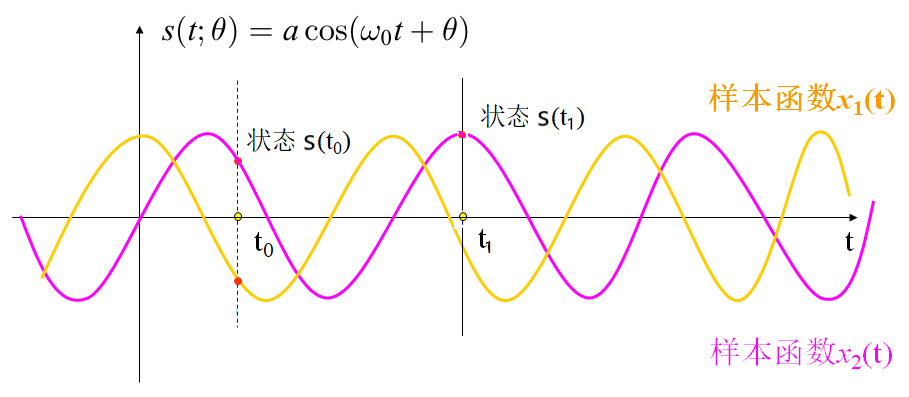
\includegraphics[scale=0.25]{sampleFun2-2}
	\column{0.4\textwidth}
	由于$a,\omega_0$为常数, 因此$r_x(t_j,t_k)$仅与采样间隔$\tau=t_j-t_k$有关, 与$\theta$无关。$\tau=0$时, 自相关函数值达到最大$\frac{a^2}{2}$。
\end{columns}
\end{frame}

\begin{frame}
\begin{block}{随机过程的自协方差函数$c_x(t_j,t_k)$}
\begin{align*}
c_x(t_j,t_k)&\mathop{=}^{def}E[((x(t_j)-\mu_x(t_j)(x(t_k)-\mu_x(t_k)]\\
&=\int_{-\infty}^{\infty}\int_{-\infty}^{\infty}(x_j-\mu_x(t_j))(x_k-\mu_x(t_k))p(x_j,x_k;t_j,t_k)dx_idx_k
\end{align*}
\end{block}
随机过程的自协方差函数$c_x(t_j,t_k)$可以理解为它的两个随机变量$x(t_j)$与$x(t_k)$之间的相关程度的度量。\\
而随机过程的自相关函数$r_x(t_j,t_k)$可以理解为它的两个随机变量$x(t_j)$与$x(t_k)$之间\textbf{含有均值}时的相关程度的度量。\\
它们的自相关系数定义为
\[\rho_x(t_j,t_k)\mathop{=}^{def}\frac{c_x(t_j,t_k)}{\sigma_x(t_j)\sigma_x(t_k)}\]
易证
\[c_x(t_j,t_k)=r_x(t_j,t_k)-\mu_x(t_j)\mu_x(t_k),\quad c_x(t,t)=\sigma_x^2(t)\]
\end{frame}

\begin{frame}{随机过程的统计平均量之间的关系}
\small
\begin{itemize}
	\item 随机过程的均值$\mu_x(t)$: 是随机过程的\textbf{所有样本函数}在时刻$t$的函数值的统计平均值。$\mu_x(t)$表示了随机过程$x(t)$在各个时刻的摆动中心。
	\item 方差$\sigma_x^2(t)$表示随机过程在$t$时刻取其值\textbf{偏离其均值}$\mu_x(t)$的离散程度。
	\item 随机过程的自相关函数$r_x(t_j,t_k)$可以理解为它的两个随机变量$x(t_j)$与$x(t_k)$之间\textbf{含有均值}时的相关程度的度量。
	\item 随机过程的自协方差函数$c_x(t_j,t_k)$可以理解为它的两个随机变量$x(t_j)$与$x(t_k)$之间的相关程度的度量。
\end{itemize}
\[c_x(t_j,t_k)=r_x(t_j,t_k)-\mu_x(t_j)\mu_x(t_k),\quad c_x(t,t)=\sigma_x^2(t)\]
\begin{columns}
	\column{0.6\textwidth}
	均值$\mu_x(t)$,均方值$\varphi_x^2(t)$,方差$\delta_x^2(t)$之间的关系:
	\[\sigma_x^2(t)=\varphi_x^2(t)-\mu_x^2(t)\]
	\column{0.3\textwidth}
	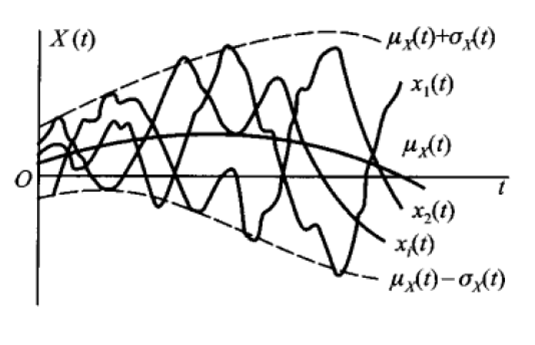
\includegraphics[scale=0.35]{delta}
\end{columns}
\end{frame}

\begin{frame}
\begin{block}{随机过程的互相关函数$r_{xy}(t_j,t_k)$}
对于两个随机过程$x(t)$和$y(t)$, 其互相关函数定义为
\begin{align*}
r_{xy}(t_j,t_k) &\mathop{=}^{def}E[x(t_j)y(t_k)]\\
&=\int_{-\infty}^{\infty}\int_{-\infty}^{\infty}x_jy_kp(x_j,t_j;y_k,t_k)dx_jdy_k
\end{align*}
式中, $p(x_j,t_j;y_k,t_k)$是$x(t)$与$y(t)$的二维混合概率密度函数。
\end{block}
\end{frame}

\begin{frame}
\begin{block}{随机过程的互协方差函数$c_{xy}(t_j,t_k)$}
\begin{align*}
c_{xy}(t_j,t_k)&\mathop{=}^{def}E[(x(t_j)-\mu_x(t_j))(y(t_k)-\mu_y(t_k))]\\
&=\int_{-\infty}^{\infty}\int_{-\infty}^{\infty}(x_j-\mu_x(t_j))(y_k-\mu_x(t_k))p(x_j,t_j;x_k,t_k)dx_jdy_k
\end{align*}
\end{block}
随机过程$x(t)$和$y(t)$的互协方差函数$c_{xy}(t_j,t_k)$可以理解为它们各自的随机变量$x(t_j)$与$y(t_k)$之间的相关程度, 实际上表示两个随机过程$x(t)$与$y(t)$之间的相关程度。它们的互相关系数定义为
\[\rho_{xy}(t_j,t_k)\mathop{=}^{def}\frac{c_{xy}(t_j,t_k)}{\sigma_x(t_j)\sigma_y(t_k)}\]
易证
\[c_{xy}(t_j,t_k)=r_{xy}(t_j,t_k)-\mu_x(t_j)\mu_y(t_k)\]
\end{frame}

\section{随机过程的平稳性}

\begin{frame}
\begin{definition}[广义平稳随机过程,简称平稳随机过程]
随机过程$x(t)$的平均统计量满足
\begin{enumerate}
\item $x(t)$的均值是与时间$t$无关的常数,即
\[E[x(t)]=\mu_x\]
\item $x(t)$的自相关函数只取决于时间间隔$\tau=t_k-t_j$,而与时间的起始时刻无关,即
\[E[x(t_j)x(t_k)]=E[x(t_j)x(t_j+\tau)]=r_x(\tau) \]
\end{enumerate}
\end{definition}
平稳随机过程$x(t)$自相关函数$r_x(t_k-t_j)$仅取决于时间间隔$(t_k-t_j)$,而与时间的起始时刻无关。$E[x(t_j)x(t_k)]=r_x[t_k-t_j]$
\end{frame}

\begin{frame}{平稳随机过程的统计平均量之间的关系}
平稳随机过程x(t)的均值$\mu_x$, 均方值$\varphi_x^2$, 方差$\sigma_x^2$,自相关函数$r_x(\tau)$,自协方差函数$c_x(\tau)$之间的关系
\begin{align*}
&\sigma_x^2=\varphi_x^2-\mu_x^2\\
&r_x(\tau)=r_x(-\tau)\\
&c_x(\tau)=r_x(\tau)-\mu_x^2\\
&c_x(\tau)=c_x(-\tau)\\
&\varphi_x^2=r_x(0)\\
&\sigma_x^2=c_x(0)\\
&r_x(0)\ge|r_x(\tau)|, \tau\ne 0\\
&c_x(0)\ge|c_x(\tau)|, \tau\ne 0
\end{align*}
\end{frame}

\begin{frame}[shrink]
\begin{example}
	假定平稳随机过程$x(t)$是周期的, 周期为$T$, 即
	\[x(t)=x(t+T) \]
	证明其自相关函数$r_x(\tau)$也是以$T$为周期的, 即
	\[r_x(\tau)=r_x(\tau+T) \]
\end{example}
\begin{proof}
	因为
	\begin{align*}
	r_x(\tau)&=E[x(t)x(t+\tau)]\\
	&=E[x(t)x(t+\tau+T)]&& \text{by } x(t+\tau)=x(t+\tau+T)\\
	&=r_x(\tau+T)
	\end{align*}
	所以, 自相关函数$r_x(\tau)$也是以$T$为周期的。
\end{proof}
\end{frame}

\begin{frame}
\begin{definition}[联合平稳随机过程]
设$x(t)$和$y(t)$分别是两个平稳的随机过程, 如果对于任意的$\Delta t$, 有$r_{xy}(t_j+\Delta t,t_k+\Delta t)=r_{xy}(t_j,t_k)$, 即互相关函数$r_{xy}(t_j,t_k)=r_{xy}(\tau),(\tau=t_k-t_j)$仅与时间间隔$\tau$有关,而与$t_j$和$t_k$无关,则称过程$x(t)$与$y(t)$是联合平稳的随机过程。
\end{definition}
\begin{block}{联合平稳随机过程$x(t)$与$y(t)$的互协方差函数}
\[c_{xy}(t_j,t_k)=c_{xy}(\tau)=r_{xy}(\tau)-\mu_x\mu_y, \tau=t_k-t_j\]
互相关系数:
\[\rho_{xy}(\tau)\mathop{=}^{def}=\frac{c_{xy}(t_j,t_k)}{\sigma_x(t_j)\sigma_y(t_k)}=\frac{c_{xy}(\tau)}{\sigma_x\sigma_y}\]
\begin{align*}
r_{xy}(\tau)&=r_{yx}(-\tau)\\
c_{xy}(\tau)&=c_{yx}(-\tau)
\end{align*}
\end{block}
\end{frame}

\section{随机过程的正交性、不相关性和统计独立性}

\begin{frame}{$x(t)$的正交性与互不相关性}
随机过程$x(t)$的任意两个不同时刻的随机变量$x(t_j)$与$x(t_k)$之间是否相互正交、互不相关和相关统计独立,表征了随机过程的重要统计特性。
\begin{definition}
	设$x(t_j),x(t_k)$是随机过程$x(t)$的任意两个不同时刻的随机变量,其均值分别为$\mu_x(t_j)$和$\mu_x(t_k)$,自相关函数为$r_x(t_j,t_k)$,自协方差函数为$c_x(t_j,t_k)$。
	\begin{enumerate}
		\item 相互正交
		$$r_x(t_j,t_k)\mathop{=}^{def}E[x(t_j)x(t_k)]=0, \quad j\ne k$$
		\item 互不相关
		$$c_x(t_j,t_k)\mathop{=}^{def}E[((x(t_j)-\mu_x(t_j)(x(t_k)-\mu_x(t_k)]=0, \quad j\ne k$$
		\item 互不相关的等价条件
		$$c_x(t_j,t_k)=r_x(t_j,t_k)-\mu_x(t_j)\mu_x(t_k), j\ne k \implies r_x(t_j,t_k)=\mu_x(t_j)\mu_x(t_k),j\ne k $$
	\end{enumerate}
	
\end{definition}
\end{frame}

\begin{frame}{平稳随机过程$x(t)$的正交性与互相关性}
\begin{definition}[]
如果$x(t)$是平稳随机过程,
\begin{enumerate}
	\item 相互正交:
	\[r_x(\tau)=0,\tau=t_k-t_j\]
	\item 互不相关:
	\[c_x(\tau)=0,\tau=t_k-t_j\]
	\item
	互不相关的等价条件
	\[r_x(\tau)=\mu_x^2,\tau=t_k-t_j\]
\end{enumerate}
\end{definition}
\end{frame}

\begin{frame}{$x(t)$的统计独立性}
\begin{definition}[]
设$x(t_1),x(t_2),\dots,x(t_N)$是随机过程$x(t)$在不同时刻$t_k(k=1,2,\dots,t_N)$的随机变量, 如果其N维联合概率密度函数对于任意的$N\ge 1$和所有时刻$t_k(k=1,2,\dots,N)$都能够表示成各自一维概率密度函数之积的形式,即
\begin{align*}
p(x_1,x_2,\dots,x_N; t_1,t_2,\dots,t_N)\\
=p(x_1;t_1)p(x_2;t_2)\cdots p(x_N;t_N)
\end{align*}
则称$x(t)$是相互统计独立的随机变量过程。
\end{definition}
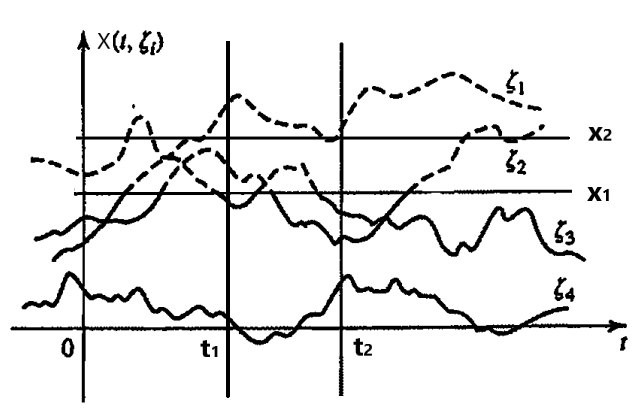
\includegraphics[scale=0.23]{sampleFun4-2}
\end{frame}

\begin{frame}{$x(t)$的正交性,不相关性以及统计独立性之间的关系}
\begin{enumerate}
\item 均值$\mu_x(t_j)=0,\mu_x(t_k)=0$则, $x(t)$相互正交$\Leftrightarrow$互不相关\\
\item $x(t)$相互统计独立$\Rightarrow$互不相关
\item $x(t)$互不相关$\nRightarrow$相互统计独立。但是若$x(t)$服从联合高斯分布,则互不相关$\Leftrightarrow$相互统计独立
\end{enumerate}
第1条可由$x(t)$互不相关的等价条件$r_x(t_j,t_k)=\mu_x(t_j)\mu_x(t_k),j\ne k $直接导出。
现证明第2条,第3条的证明见后。
\end{frame}

\begin{frame}
证明:如果$x(t)$是一个相互统计独立随机变量过程,则它一定是一个互不相关随机变量过程。
\begin{proof}%[caption]
	设$x(t_j)$与$x(t_k)$是相互统计独立的, 则其自相关函数为
	\begin{align*}
	r_x(t_j,t_k)&\mathop{=}^{def}E[x(t_j)x(t_k)]\\
	&=\int_{-\infty}^{\infty}\int_{-\infty}^{\infty}x_jx_kp(x_j,x_k;t_j,t_k)dx_jdx_k\\
	&=\int_{-\infty}^{\infty}x_jp(x_j;t_j)dx_j\int_{-\infty}^{\infty}x_jp(x_k;t_k)dx_k\\
	&=\mu_x(t_j)\mu_x(t_k)
	\end{align*}
	这正是$x(t)$互不相关的等价条件$r_x(t_j,t_k)=\mu_x(t_j)\mu_x(t_k),j\ne k $,所以$x(t)$统计独立$\implies$ 互不相关
\end{proof}
由证明过程,可以得到: \textcolor{blue}{$x(t)$相互统计独立,则,$E[x(t_j)x(t_k)]=E[x(t_j)]E[x(t_k)]$}
\end{frame}

\begin{frame}{两个随机过程$x(t), y(t)$的正交性与互不相关性}
设$x(t_j)$是$x(t)$在$t_j$时刻的随机变量, $y(t_k)$是$y(t)$在$t_k$时刻的随机变量。
\begin{definition}
	$x(t)$在$t_j$, $y(t)$在$t_k$的均值分别为$\mu_x(t_j)$和$\mu_y(t_k)$, 互相关函数为$r_{xy}(t_j,t_k)$, 互协方差函数为$c_{xy}(t_j,t_k)$。
	\begin{enumerate}
		\item 相互正交
		$$r_{xy}(t_j,t_k)\mathop{=}^{def}E[x(t_j)y(t_k)]=0, \quad j\ne k$$
		\item 互不相关
		$$c_{xy}(t_j,t_k)\mathop{=}^{def}E[((x(t_j)-\mu_x(t_j)(y(t_k)-\mu_y(t_k)]=0, \quad j\ne k$$
		\item 互不相关的等价条件
		$$c_{xy}(t_j,t_k)=r_{xy}(t_j,t_k)-\mu_x(t_j)\mu_y(t_k), j\ne k \implies r_{xy}(t_j,t_k)=\mu_x(t_j)\mu_y(t_k),j\ne k $$
	\end{enumerate}	
\end{definition}
\end{frame}

\begin{frame}{两个平稳随机过程$x(t), y(t)$的正交性与互相关性}
\begin{definition}[]
	如果$x(t), y(t)$是联合平稳的随机过程,
	\begin{enumerate}
		\item 相互正交:
		\[r_{xy}(\tau)=0,\tau=t_k-t_j\]
		\item 互不相关:
		\[c_{xy}(\tau)=0,\tau=t_k-t_j\]
		\item
		互不相关的等价条件
		\[r_{xy}(\tau)=\mu_x\mu_y,\tau=t_k-t_j\]
	\end{enumerate}
\end{definition}
\end{frame}

\begin{frame}{两个随机过程$x(t), y(t)$的统计独立性}
\begin{definition}
	如果随机过程$x(t)$和$y(t)$对任意的$N\ge 1, M\ge 1$和所有时刻$t_k(k=1,2,\dots,t_N)$与$t_k^\prime(k=1,2,\dots,M)$, 其$N+M$维联合概率密度表示为
	\begin{align*}
	p(x_1,x_2,\dots,x_N; t_1,t_2,\dots,t_N; y_1,y_2,\dots,y_N; t_1^\prime,t_2^\prime,\dots,t_M^\prime)\\
	=p(x_1,x_2,\dots,x_N; t_1,t_2,\dots,t_N)p(y_1,y_2,\dots,y_N; t_1^\prime,t_2^\prime,\dots,t_M^\prime)
	\end{align*}
	则称$x(t)$与$y(t)$是相互统计独立的两个随机变量过程。
\end{definition}
\end{frame}

\begin{frame}{相互独立的随机过程$E[x(t)y(t)]=E[x(t)]E[y(t)]$}
\begin{block}{}
	设$x(t), y(t)$是相互独立的随机过程, 则有
	\[ E[x(t)y(t)]=E[x(t)]E[y(t)]\]
	这一性质可以推广至任一两个有限个相互独立的随机变量之积的情况。
\end{block}
\begin{proof}
	\begin{align*}
	E[x(t)y(t)]&=\int_{-\infty}^{\infty}\int_{-\infty}^{\infty}xyp(x,y)dxdy\\
	&=\int_{-\infty}^{\infty}\int_{-\infty}^{\infty}xyp_x(x)p_ydxdy\\
	&=\left[\int_{-\infty}^{\infty}xp_x(x)dx\right]\left[\int_{-\infty}^{\infty}yp_y(y)dy\right]\\
	&=E[x(t)]E[y(t)]
	\end{align*}
\end{proof}
\end{frame}

\begin{frame}{$x(t),y(t)$的正交性,不相关性以及统计独立性之间的关系}
\begin{enumerate}
	\item 均值之一或同时为零, 则$x(t), y(t)$相互正交$\Leftrightarrow$互不相关\\
	\item $x(t), y(t)$相互统计独立$\Rightarrow$互不相关
	\item $x(t), y(t)$互不相关$\nRightarrow$相互统计独立。但是若$x(t), y(t)$服从联合高斯分布,则互不相关$\Leftrightarrow$相互统计独立
\end{enumerate}
\end{frame}

\begin{frame}{雷达回波信号}
\begin{example}
	设$s(t)$是雷达的发射信号, 遇到目标后的反射信号为$as(t-t_0), t_0$是信号返回的延迟时间。如果回波信号中伴有加性噪声$n(t)$, 则接收到的信号为
	\[x(t)=as(t-t_0)+n(t) \]
	\begin{enumerate}
		\item 假定$s(t)$和$n(t)$是平稳相关的, 试求互相关函数$r_{sx}(\tau)$。
		\item 如果噪声$n(t)$的均值为零, 且与$s(t)$相互统计独立, 试求互相关函数$r_{sx}(\tau)$。
	\end{enumerate}
\end{example}
\end{frame}

\begin{frame}[shrink]
解:
\begin{enumerate}
\item 假定$s(t)$和$n(t)$是平稳相关的, 试求互相关函数$r_{sx}(\tau)$。\begin{align*}
r_{sx}(\tau)&=E[s(t)x(t+\tau)] \\
&=E[s(t)(as(t-t_0+\tau)+n(t+\tau)))] &&\text{by } x(t)=as(t-t_0)+n(t)\\
&=aE[s(t)s(t-t_0+\tau)]+E[s(t)n(t+\tau)]\\
&=ar_{s}(\tau-t_0)+r_{sn}(\tau)
\end{align*}
\item 如果噪声$n(t)$的均值为零, 且与$s(t)$相互统计独立, 试求互相关函数$r_{sx}(\tau)$。
\begin{align*}
r_{sx}(\tau)&=E[s(t)x(t+\tau)] \\
&=E[s(t)(as(t-t_0+\tau)+n(t+\tau)))] &&\text{by } x(t)=as(t-t_0)+n(t)\\
&=aE[s(t)s(t-t_0+\tau)]+E[s(t)n(t+\tau)] &&\text{相互统计独立E[XY]=E[X]E[Y]}\\ 
&=aE[s(t)s(t-t_0+\tau)]+E[s(t)]E[n(t+\tau)] &&\text{确知信号$s(t)$看作常数,$E[s(t)]=s(t)$}\\ 
&=aE[s(t)s(t-t_0+\tau)]+s(t)E[n(t+\tau)] &&\text{by }E[n(t)]=0 \\
&=ar_{s}(\tau-t_0)
\end{align*}
\end{enumerate}
\end{frame}

\section{平稳随机过程的功率谱密度}

\begin{frame}{平稳随机过程的功率谱密度}
如果平稳过程$x(t)$的自相关函数$r_x(\tau)$绝对可积,即
$$\int_{-\infty}^{\infty}|r_x(\tau)|d\tau <\infty$$
则功率谱密度$P_x(\omega)$与自相关函数$r_x(\tau)$
$$P_x(\omega)=\int_{-\infty}^{\infty}r_x(\tau)e^{-j\omega\tau}d\tau,\quad -\infty<\omega<\infty$$
$$r_x(\tau)=\frac{1}{2\pi}\int_{-\infty}^{\infty}P_x(\omega)e^{j\omega\tau}d\omega,\quad -\infty<\omega<\infty$$
$P_x(\omega)$与$r_x(\tau)$构成傅里叶变换对
\end{frame}

\begin{frame}{功率谱密度主要性质}
\begin{enumerate}
	\item $P_x(\omega)$非负
			$$P_x(\omega)\ge 0$$
	\item $P_x(\omega)$是$\omega$的偶函数
			$$P_x(\omega) = P_x(-\omega)$$
	\item 当$\omega=0$或$\tau=0$时,$P_x(\omega)$与$r_x(\tau)$的变换关系是
			$$P_x(0)=\int_{-\infty}^{\infty}r_x(\tau)d\tau$$
			$$r_x(0)=\frac{1}{2\pi}\int_{-\infty}^{\infty}P_x(\omega)d\omega$$	
\end{enumerate}
\begin{block}{第3条表明}
	$x(t)$的功率谱密度的零频率分量等于$x(t)$的自相关函数曲线下的总面积。因为$r_x(0)=E[x^2(t)]$, 所以, $x(t)$的功率谱密度曲线下的总面积等于$x(t)$的平均功率。
\end{block}
\end{frame}

\section{高斯噪声、白噪声、高斯白噪声和有色噪声}

\begin{frame}{高斯(正态)分布随机变量}
均值$\mu_x$,方差为$\sigma_x^2$的高斯分布随机变量$x(\xi)$概率密度函数$p(x)$表示为
\[p(x)=\left(\frac{1}{2\pi\sigma_x^2}\right)^{1/2}\exp\left[-\frac{(x-\mu_x)^2}{2\sigma_x^2}\right] \]
\begin{columns}
	\column{0.5\textwidth}%<1->
	\begin{block}{特性}
		高斯分布随机变量$x(\xi)$的概率密度函数$p(x)$完全由它的均值$\mu_x$和方差$\sigma_x^2$来表示。记为$x(\xi)\sim\mathcal{N}(\mu_x,\sigma_x^2)$
	\end{block}
	\column{0.4\textwidth}
	\begin{figure}[!h]
		\centering
		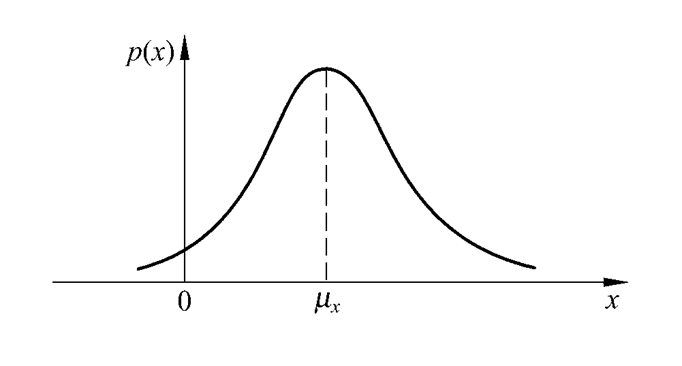
\includegraphics[width=4cm]{Gaussian}
		\caption{高斯(正态)分布随机变量的PDF曲线$\mu_x>0$}
	\end{figure}
    \tiny PDF---概率密度函数(Probability Density Function)
\end{columns}
\end{frame}

\begin{frame}{标准高斯(正态)分布随机变量}
归一化处理$x(\xi)\sim\mathcal{N}(\mu_x,\sigma_x^2)$为$x(\xi)\sim\mathcal{N}(0,1)$, 令
\[u(\xi)=\frac{x(\xi)-\mu_x}{\sigma_x}\]
有
\[p(x)=\left(\frac{1}{2\pi}\right)^{1/2}\exp\left(-\frac{u^2}{2}\right) \]
\begin{columns}
\column{0.4\textwidth}%<1->
\begin{figure}[!h]
	\centering
	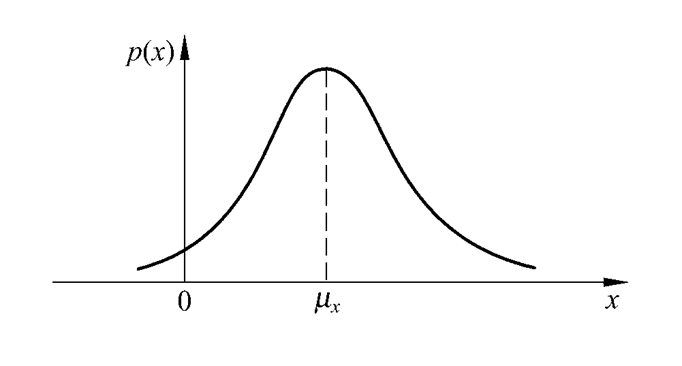
\includegraphics[width=4cm]{Gaussian}
	\caption{高斯(正态)分布随机变量的PDF曲线$\mu_x>0$}
\end{figure}
\column{0.4\textwidth}
\begin{figure}[!h]
	\centering
	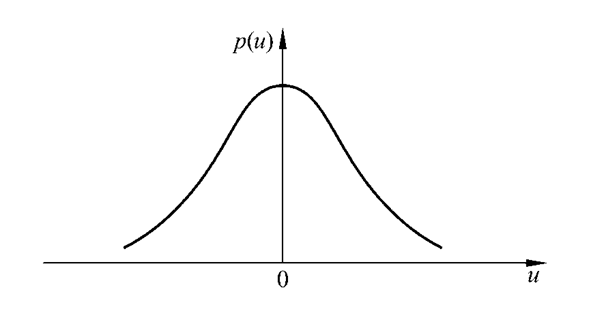
\includegraphics[width=4cm]{GaussianN}
	\caption{标准高斯(正态)分布随机变量的PDF曲线$\mu_x=0$}
\end{figure}
\end{columns}
\end{frame}

\begin{frame}{标准高斯(正态)分布随机变量}
\begin{columns}
\column{0.6\textwidth}%<1->
标准高斯分布随机变量的一维累积分布函数(正态概率积分)定义为
\[\Phi(x)\mathop{=}^{def}\int_{-\infty}^{x}\left(\frac{1}{2\pi}\right)^{1/2}\exp\left(-\frac{u^2}{2}\right)du \]
它的互补累积分布函数是标准高斯分布的右尾积分,即
\[Q(x)=1-\Phi(x)\mathop{=}^{def}\int_{x}^{\infty}\left(\frac{1}{2\pi}\right)^{1/2}\exp\left(-\frac{u^2}{2}\right)du \]
\column{0.4\textwidth}
\begin{figure}[!h]
\centering
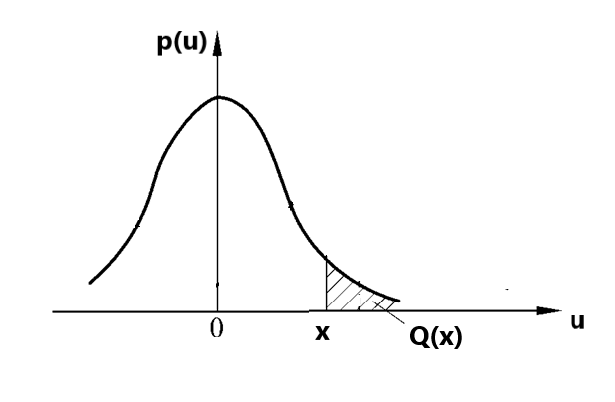
\includegraphics[width=4cm]{Qx}\\
\caption{标准高斯(正态)分布的右尾积分$Q(x)$}
\end{figure}
\end{columns}
\end{frame}

\begin{frame}{高斯噪声的统计描述(1)}
\begin{definition}[高斯噪声]
	噪声$n(t)$, 对任意$N\ge 1$和所有时刻$t_k$, 随机变量$n(t_k)$服从高斯分布,则$n(t)$为一个高斯噪声随机变量过程,简称高斯噪声过程或高斯噪声。
\end{definition}
\begin{block}{高斯噪声一维概率密度函数}
	\[p(n_k;t_k)=(\frac{1}{2\pi\sigma_{n_k}^2})^{1/2}\exp\left[-\frac{(n_k-\mu_{n_k})^2}{2\sigma_{n_k}^2}\right] \]
	其中,$\mu_{n_k}$为$n(t_k)$的均值, $\sigma_{n_k}$为$n(t_k)$的方差。
\end{block}
\end{frame}

\begin{frame}{高斯噪声的统计描述(2)}
\begin{block}{高斯噪声N维联合概率密度函数}
高斯噪声的N维矢量记为
\[(\bm{n;t})=(n(t_1),n(t_2),\cdots,n(t_N))^T \]
其N维联合概率密度函数为
\begin{align*}
p(\bm{n;t})&=p(n_1,n_2,\cdots,n_N; t_1,t_2,\cdots,t_N)\\
&=\frac{1}{(2\pi)^{N/2}|\bm{C_n}|^{1/2}}\exp\left[-\frac{1}{2}(\bm{n-\mu_n})^T\bm{C_n}^{-1}(\bm{n-\mu_n})\right]
\end{align*}

其中,$\bm{\mu_{n}}$是高斯随机矢量$(\bm{n;t})$的均值矢量,$\bm{C_n}$为协方差矩阵。
即
$$\bm{\mu_n}=(\mu_{n_1},\mu_{n_2},\dots,\mu_{n_N})^T$$
$$\mu_{n_k}=E[n(t_k)]$$
\end{block}
\end{frame}

\begin{frame}
$\bm{C_n}$是高斯随机矢量$\bm{(n;t)}$的协方差
$$
\bm{C_n}=\left[
\begin{matrix}
C_{n_1n_1} & C_{n_1n_2} & \cdots &C_{n_1n_N} \\
C_{n_2n_1} & C_{n_2n_2} & \cdots &C_{n_2n_N} \\
\vdots     &  \vdots    &        &\vdots \\
C_{n_Nn_1} & C_{n_Nn_2} & \cdots &C_{n_Nn_N} \\
\end{matrix}
\right]
$$
其中$C_{n_jn_k}=E[(n(t_j)-\mu_{n_j})(n(t_k)-\mu_{n_k})]=c_{n_k}c_(n_j)$\\
$|\bm{C_n}|$是$\bm{C_n}$的行列式,$\bm{C_n^{-1}}$是$\bm{C_n}$的逆矩阵。
\end{frame}

\begin{frame}{高斯变量$n(t_k)$互不相关$\Leftrightarrow$相互统计独立}
	\begin{block}{不相关性与统计独立性}
		互不相关$\nRightarrow$相互统计独立。但是若$x(t)$服从联合高斯分布,则互不相关$\Leftrightarrow$相互统计独立
	\end{block}
\textbf{证明:} 设高斯随机矢量$\bm{(n;t)}$中的$n(t_j)$与$n(t_k)(j\ne k)$互不相关,即$C_{n_jn_k}=C_{n_kn_j}=0(j\ne k)$, 若记$\sigma_{n_k}^2\mathop{=}\limits^{def}C_{n_kn_k}$,则协方差矩阵$C_n$和$\bm{C_n^{-1}}$分别为
	\begin{columns}
		\column{0.5\textwidth}
		$$
		\bm{C_n}=\left[
		\begin{matrix}
		\sigma_{n_1}^2 &  0                 & \cdots & 0\\
		0              &  \sigma_{n_2}^2  & \cdots & 0\\
		\vdots         &  \vdots            &        &\vdots \\
		0              &  0                 & \cdots &\sigma_{n_N}^2\\
		\end{matrix}
		\right]
		$$
		\column{0.5\textwidth}
		$$\bm{C_n^{-1}}=\left[
		\begin{matrix}
		(\sigma_{n_1}^2)^{-1} &  0                 & \cdots & 0\\
		0              &  (\sigma_{n_2}^2)^{-1}  & \cdots & 0\\
		\vdots         &  \vdots            &        &\vdots \\
		0              &  0                 & \cdots &(\sigma_{n_N}^2)^{-1}\\
		\end{matrix}
		\right]
		$$
	\end{columns}
	而$|\bm{C_n}|^{1/2}$为: $|\bm{C_n}|^{1/2}=\prod\limits_{k=1}^{N}\sigma_{n_k}$
\end{frame}

\begin{frame}
	因此,高斯噪声$n(t)$的N维联合概率密度函数为
	\begin{align*}
	p(\bm{n;t})&=p(n_1,n_2,\cdots,n_N; t_1,t_2,\cdots,t_N)\\
	&=\frac{1}{(2\pi)^{N/2}|\bm{C_n}|^{1/2}}\exp\left[-\frac{1}{2}(\bm{n-\mu_n})^T\bm{C_n}^{-1}(\bm{n-\mu_n})\right]\\
	&=\frac{1}{(2\pi)^{N/2}|\prod\limits_{k=1}^{N}\sigma_{n_k}}\exp\left[-\sum\limits_{k=1}^{N}\frac{(n_k-\mu_{n_k})^2}{2\sigma_{n_k}^2}\right]\\
	&=\prod\limits_{k=1}^{N}\left(\frac{1}{2\pi\sigma_{n_k}}\right)^{1/2}\exp\left[-\frac{(n_k-\mu_{n_k})^2}{2\sigma_{n_k}^2}\right]\\
	&=p(x_1;t_1)p(x_2;t_2)\cdots p(x_N;t_N)
	\end{align*}
	表明$n(t)$的N维联合概率密度函数表示成各自一维概率密度函数之积的形式,即是统计独立性的定义。因此,\textbf{N个高斯随机变量$n(t_k)(k=1,2,\dots,t_N)$互不相关$\Rightarrow$相互统计独立}; 结合之前的结论``相互统计独立的随机变量$\Rightarrow$互不相关''。所以, \textbf{
	N个高斯随机变量$n(t_k)(k=1,2,\dots,t_N)$互不相关$\Leftrightarrow$相互统计独立}。
\end{frame}

\begin{frame}{高斯随机变量的线性组合仍然是高斯随机变量}
\begin{enumerate}
	\item 若$x_k(\xi)\sim\mathcal{N}(\mu_{x_k},\sigma_{x_k}^2)(k=1,2,\dots,N)$,且它们相互统计独立,则它们的和
	\[x(\xi)=\sum\limits_{k=1}^{N}x_k(\xi) \]
	是高斯随机变量,且有$x_k(\xi)\sim\mathcal{N}(\mu_x,\sigma_x^2)$,其中
	$\mu_x=\sum\limits_{k=1}^N\mu_{x_k},\sigma_x^2=\sum\limits_{k=1}^N\sigma_{x_k}^2$
	\item 更一般地,任意有限N个高斯随机变量$x_k(\xi)(k=1,2,\dots,N)$的线性组合
	\[x(\xi)=\sum\limits_{k=1}^{N}a_kx_k(\xi) \]
	仍然是高斯随机变量,且有$x_k(\xi)\sim\mathcal{N}(\mu_x,\sigma_x^2)$,其中
	$\mu_x=\sum\limits_{k=1}^Na_k\mu_{x_k},\sigma_x^2=\sum\limits_{j=1}^N\sum\limits_{k=1}^Na_ja_kc_{x_kx_j}$\\
	式中,协方差函数$c_{x_jx_k}=E[(x_j(\xi)-\mu_{x_j})(x_k(\xi)-\mu_{x_k})]=c_{x_kx_j},\mu_{x_k}=E[x_k(\xi)]$
\end{enumerate}
\end{frame}

\begin{frame}
\begin{example}
	设随机变量$y$与$x$之间为线性关系$y=ax+b,a,b$为常数,且$a\ne 0$。已知随机变量$x$服从高斯分布,即
	\[p(x)=\left(\frac{1}{2\pi\sigma_x^2}\right)^{1/2}\exp\left[-\frac{(x-\mu_x)^2}{2\sigma_x^2}\right] \]
	证明随机变量$y$是服从均值为$a\mu_x+b$, 方差为$a^2\sigma_x^2$的高斯分布。
\end{example}
\end{frame}

\begin{frame}
\begin{proof}
证法I: 雅可比变换法
\begin{align*}
&\text{因为}\qquad  y=ax+b \\
&\text{所以,反函数为}\qquad  x=\frac{y-b}{a} \\
&\text{且有}\qquad  \frac{dx}{dy}=\frac{1}{a} \\
&\text{于是,由一维雅可比变换,得}  \\
&p(y)=\left(\frac{1}{2\pi\sigma_x^2}\right)^{1/2}\exp\left[-\frac{(\frac{y-b}{a}-\mu_x)^2}{2\sigma_x^2}\right]\left|\frac{1}{a}\right| \\
&=\left(\frac{1}{2\pi  a^2\sigma_x^2}\right)^{1/2}\exp\left[-\frac{(y-(a\mu_x+b))^2}{2a^2\sigma_x^2}\right]  
\end{align*}
所以,随机变量$y$是服从均值为$a\mu_x+b$, 方差为$a^2\sigma_x^2$的高斯分布。
\end{proof}
\end{frame}

\begin{frame}
\begin{proof}
证法II: 利用高斯随机变量的特性来证明\\
因为  $y=ax+b$ \\
是高斯随机变量$x$的线性变换,所以$y$仍然是高斯随机变量。\\
其均值$\mu_y$和方差$\sigma_y^2$分别为
\begin{align*}
\mu_y&=E(y)=E(ax+b)=aE(x)+b\\
&=a\mu_x+b\\
\sigma_y^2&=E[(y-\mu_y)^2]=E[(ax+b-a\mu_x-b)^2]\\
&=a^2E[(x-\mu_x)^2]\\
&=a^2\sigma_x^2
\end{align*}
所以,随机变量$y$是服从均值为$a\mu_x+b$, 方差为$a^2\sigma_x^2$的高斯分布。
\end{proof}
\end{frame}

\begin{frame}{白噪声}
\small
%白噪声的频域,时域描述:
\begin{columns}%0.6 0.4表示相对比例
	\column{0.6\textwidth}
	\begin{block}{频域---白噪声的功率谱密度}
	功率谱密度均匀分布在整个频率轴上: $p_n(\omega)=\frac{N_0}{2},\quad -\infty<\omega< \infty, N_0$是常数\\
	也可以按正半轴上的频域定义: $p_n(\omega)=N_0,\quad 0<\omega<\infty, N_0$是常数
	\end{block}
    \column{0.3\textwidth}
    \includegraphics[scale=0.3]{WhiteNoise2}
\end{columns}

\begin{columns}%0.6 0.4表示相对比例
	\column{0.6\textwidth}
	\begin{block}{时域---白噪声的自相关函数}
	均值为零、自相关函数$r_n(\tau)$为$\delta$的噪声随机过程: $r_n(\tau)=IFT[\frac{N_0}{2}]=\frac{N_0}{2}\delta(\tau)$
	\end{block}
	\column{0.3\textwidth}
	\includegraphics[scale=0.3]{WhiteNoise1}
\end{columns}
\begin{block}{意义}
	白噪声是一种理想化的数学模型,由于其功率谱密度在整个频域上均匀分布,所以其能量是无限的,实际上是不存在的。但是由于我们所采用的系统相对于整个频率轴来说是窄带系统,只要认为频谱是均匀分布的,能够在数学上带来很大方便。
\end{block}
\end{frame}

\begin{frame}{白噪声特性}
\includegraphics[scale=0.4]{WhiteNoise}
\begin{block}{白噪声$n(t)$重要特性}
	\begin{itemize}
		\item 白噪声在频域上其功率谱密度是均匀分布的;
		\item 时域上自相关函数$r_n(\tau)$是$\delta$函数: $r_n(\tau)=IFT[\frac{N_0}{2}]=\frac{N_0}{2}\delta(\tau)$
		\item 任意两个不同时刻的随机变量$n(t_j)$与$n(t_k),(\tau=t_j-t_k\ne 0)$是不相关的:\\
		$r_n(t_j,t_k)=r_n(\tau)=E[n(t_j)n(t_k)]=0,(\tau=t_j-t_k\ne 0)$。
		\item 由于$\delta$---函数的筛选性: $\int_{-\infty}^{\infty}\delta(t-t_0)f(t)dt=f(t_0)$,有\\
		$\int_{-\infty}^{\infty}r_n(t-t_0)f(t)dt=f(t_0)=\frac{N_0}{2}\int_{-\infty}^{\infty}\delta(t-t_0)f(t)dt=\frac{N_0}{2}f(t_0)$
	\end{itemize}	
\end{block}
\end{frame}

\begin{frame}{高斯白噪声}
\begin{block}{高斯白噪声$n(t)$重要特性---高斯随机变量+白噪声}
	\begin{itemize}
		\item 高斯白噪声在频域上其功率谱密度是均匀分布的;
		\item \textbf{时域上概率密度函数是高斯分布的。(白噪声对此没有明确限制)}
		\item 时域上自相关函数$r_n(\tau)$是$\delta$函数: $r_n(\tau)=IFT[\frac{N_0}{2}]=\frac{N_0}{2}\delta(\tau)$
		\item 任意两个不同时刻的随机变量$n(t_j)$与$n(t_k),(\tau=t_j-t_k\ne 0)$是不相关的,\textbf{并且是统计独立的}:\\
		$r_n(t_j,t_k)=r_n(\tau)=E[n(t_j)n(t_k)]=E[n(t_j)]E[n_k(t_k)]=0,(\tau=t_j-t_k\ne 0)$。
		\item 由$\delta$---函数的筛选性: $\int_{-\infty}^{\infty}\delta(t-t_0)f(t)dt=f(t_0)$,有\\
		$\int_{-\infty}^{\infty}r_n(t-t_0)f(t)dt=f(t_0)=\frac{N_0}{2}\int_{-\infty}^{\infty}\delta(t-t_0)f(t)dt=\frac{N_0}{2}f(t_0)$
	\end{itemize}	
\end{block}
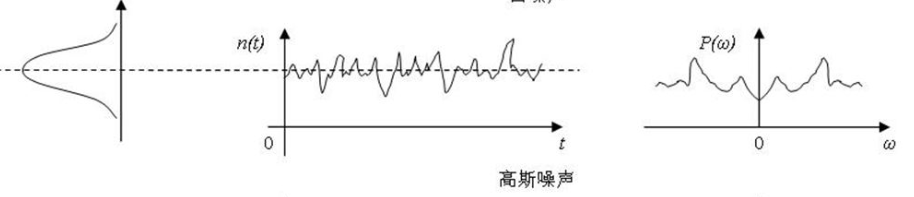
\includegraphics[scale=0.4]{WhiteGaussianNoise}
\end{frame}

\begin{frame}{有色噪声}
如果噪声过程$n(t)$的功率谱密度在频域上的分布是不均匀的,则称其为有色噪声。
\begin{block}{有色噪声的功率谱密度}
	\[P_n(f) =P_0\exp\left[-\frac{(f-f_0)^2}{2\sigma_f^2}\right]\]
	均值$f_0$代表频谱的中心频率,方差$\sigma_f^2$反映噪声的谱宽度。$\omega=2\pi f$
\end{block}
\end{frame}

\begin{frame}[shrink]
\frametitle{ch2.信号检测与估计理论的基础知识}
\tableofcontents[hideallsubsections]
\end{frame}


